
\chapter{Current Techniques}
The ultimate goal of this project is to provide a new set of tools
for analyzing FMRI data. Whereas SPM techniques have been highly 
successful at finding macroscopic regions of activation, linear 
modeling can carry significant bias error due to lack of model
flexibility. While adding parameters can significantly increase
error due to model variance, this effect should be mitigated first
by the use of a highly constrained model based on first principals
and also by the
calculation of a full posterior distribution, rather than a single
estimate. The
purpose of this paper is thus to evaluate the potential of using
a particle filter along with the BOLD model to derive physical 
parameters. In so doing, we hope to be able to show that one or more
parameters are a suitable replacement for estimating voxel 
activation from a standard FMRI image. We also hope to show that 
estimated posterior distribution of the parameters, derived from
the particle filter, is able to provide an accurate measure of the
confidence interval.

\section{Nonlinear Least Squares}
\label{sec:Nonlinear Least Squares}
Although there are certainly benefits to using a derived model, rather
than a purely empirical model, there are serious implications. The
first problem is that all the powerful classical techniques of gradient
descent are off limits; since the model is a true nonlinear dynamical
system with no closed form solution. The implication of this is that
the calculation of a Jacobian for residuals won't work; and thus powerful
techniques such as the Gauss-Newton method, which are helpful in many nonlinear
problems, are off limits. Additionally, a gradient descent is difficult to
perform without the ability to form partials of the output with respect
to all the parameters. 

Although anything requiring a Jacobian is out, there are other heuristic
techniques that could potentially illuminate the BOLD response. 
Simulated Annealing (SA) is a common method of optimizing high dimensional
regression problems. The idea is to pick a random start, and then
at each iteration pick a random nearby point, and if that point is
below some energy constraint (energy is a function of the residual), 
called the temperature, the algorithm moves
to that point and continues with the next iteration. The temperature
is slowly lowered until no nearby points below the temperature can
be found (or the temperature drops below the current point). There are
variations of this, for instance it is common to require every movement
to be in the downward direction (in terms of energy). Like most nonlinear
optimization problems, there is no guarantee of an optimal solution,
although the longer the algorithm is allowed to run, the better the solution
will get. Since every step requires an entirely new run of the 
BOLD model, it can be extremely time consuming, which is why we are
not using it here.

\begin{algorithm}
\caption{Simulated Annealing Algorithm}
\label{alg:Simulated Annealing}
\begin{algorithmic}
\STATE Initialize $\Theta$, or if there exists a decent estimate start there
\STATE Initialize temperature, T to value above initial energy
\WHILE{$E(\Theta) < T$}
    \REPEAT
        \STATE Pick $\theta$ near $\Theta$
        \STATE Calculate energy, $E$, of $\theta$
    \UNTIL{$E > T$}
    \STATE Move to new estimate: set $\Theta = \theta$
\ENDWHILE
\end{algorithmic}
\end{algorithm}

[simulated annealing image?]

Another potential method of interest is the use of Genetic Algorithms
(GA). Genetic algorithms are similar to Simulated Annealing, in
that they randomly move to better solutions based on a cost function.
However; in genetic algorithms a single point estimate isn't used. Instead
a population of estimates is generated, each with distinct parameters,
and then each set of parameters is rated with a fitness function. Parameter
sets that are good get a higher "fitness"; then new parameter sets are generated by 
randomly combining pieces of the old parameter sets. The pieces are typically
chosen at a rate proportional to the fitness of the donor; thus "fit"
parameter sets tend to pass on their properties. In addition to this,
random mutations may be introduced that come from no existing parent. 
The new generation is then rated with the fitness function again, and
the entire process starts over. The stop condition for a genetic algorithm
is typically based on some threshold for fitness or a maximum number 
of generations. This is problematic, since it doesn't really provide 
any guarantee of even reaching a local minima, although in practice
it can be quite effective.

[genetic algorithm picture]

\begin{algorithm}
\caption{Genetic Algorithm}
\label{alg:Genetic Algorithm}
\begin{algorithmic}
\STATE Initialize $N$ estimates, $E = \{\Theta_0, \Theta_1, ... \Theta_N\}$
\FOR{G generations}
    \STATE Calculate fitness for each $\Theta$, Ex. for residual $R$, $1/R$ or, $e^{-R}$
    \FOR{$i$ in $N$}
        \STATE Randomly select two parents (with higher probability for more fit $\Theta$'s)
        \STATE Randomly merge parts of the two parents to form a new $\Theta_i$
        \STATE At some low probability change one or two parameters in $\Theta_i$
    \ENDFOR
\ENDFOR
\end{algorithmic}
\end{algorithm}

Although both these methods can be highly effective, they have the downside of
requiring large amounts of computation time. In this case of the BOLD model,
each time the energy or fitness needs to be calculated, a large number of cycles
must be spent re-simulating the BOLD model for the set of parameters. As we'll
discuss in \autoref{sec:Particle Filters}, the Particle Filter method is able
to circumvent this re-calculation to some degree.

It would not be unreasonable at this point to back off and work with a linearized
or more static version of the model. This is the approach taken by the
standard General Linear Model discussed in \autoref{sec:Current Techniques General Linear Model}.

\section{Basic Statistical Parametric Mapping}
Although not strictly the same thing as parameter calculation from 
FMRI, activation detection is very similar. In fact, estimation of 
parameters is somewhat a generalization of the idea of activation detection.
Therefore, it is important to draw a comparison between the methods proposed
in this thesis with existing methods of activation detection.

The most basic method of analyzing FMRI data is through a standard T-test
between "resting state" and "active state" samples. This is done by 
taking the average and variance of the inactive period, and the 
period during which the stimulus was activate separately then treating 
them both as gaussian distributions.
If they are in fact Gaussian distributions, then a basic t-test will
give the probability that the samples came from the same distribution
(the null hypothesis). Of course, this test is fraught with problems; even if
the drift mentioned earlier has been removed, there is little reason
to believe that the noise is Gaussian, or even stable. Additionally, 
even if the noise were Gaussian, a t-test with a p-value of .05 over
50000 or more samples is on average going to generate $.05*50000$ false
positives. To compensate for this, bonferoni correction, also known as
multiple comparison tests are performed; essentially p-values are 
divided by the number of independent
tests being run. This, however, leads to extremely low p-values, so
low that it would be impossible for any biological system to satisfy. To
compensate, a Gaussian kernel is applied to the image, thus reducing
variance (and thus separating the active and inactive distributions)
as well as decreasing the effective number of voxels. Since t-tests are
now no longer being applied to n <I need to define n> independent voxels,
the factor by which the p-value must be divided by can be decreased.
<Do I need to mathematically define all this?> The derivation and application
of random field theory, and its use can be found in various papers \cite{Worsley2004}.

\subsection{General Linear Model}
\label{sec:Current Techniques General Linear Model}
The most used form of FMRI analysis is Statistical Parametric
Mapping, but is able to account for several different levels or types
of stimulus (see \cite{Hofmann1997}). By using hierarchical models
the output signal timeseries is considered the weighted
sum of the various input timeseries. Essentially every experimental factor
is considered as another level inputs (ex. different type of stimulus,
different run with the same patient, different patient). 
The equation for a general linear model is then
\begin{equation}
Y(t) = X(t)\beta + \epsilon(t)
\end{equation}
where $Y(t)$ is the smoothed or detrended timeseries of measurements,
$X(t)$ is a row vector of input, $\beta$ is a column vector of weights,
and $\epsilon$ is the error. Thus for every time, the measurement is
assumed to be a weighted sum of the columns of $X$ plus some error. The calculation
of $\beta$ is then performed using a maximum likelihood or gradient descent search 
to minimize the error.

\begin{figure}
\caption{GLM todo}
\label{fig:GLM}
\end{figure}

It is well known of course that a square wave stimulus does not result in a square wave
in the activation of brain regions. Thus, various methods are used to 
smooth the columns of $X$, and thus bandlimit the input. 
The best technique is convolving the stimulus input with a Hemodynamic 
Response Function (HRF), which mimics the basic shape of BOLD activation, including a delay
due to rise time and fall time. The downside of this method, however is that 
the shape of the Hemodynamic Signal is static, meaning the same Hemodynamic Function is
used for every region of the brain, and $Y(t)$ must linear combination 
of scalar the columns of $X$ to be appropriately identified. Additionally, 
it is well known that different Hemodynamic Response Functions are necessary for different 
regions of the brain. The "Canonical" HRF that is most used, has been fitted
for the visual cortex. Thus the shape of the HRF may differ significantly in
terms of onset and fall time in other areas of the brain \cite{Handwerker2004}. 
The inability to
fit parameters other than scale certainly hinders SPM's
ability to locate voxels that do not conform to the "canonical" hemodynamic 
response function. If there are different HRF's for different regions 
of the brain, might there also be more subtle differences even within
a particular region? It seems reasonable to think so. As a result, the 
most common use of SPM will be heavily biased toward the visual cortex.

\begin{figure}
\caption{Hemodynamic Response Function todo}
\label{fig:HRF}
\end{figure}

The GLM is extremely powerful at determining the linear dependence of
a set of regressors on the output. Unfortunately, there is significant evidence
that many of these dependencies are nonlinear, which means they may be
difficult or impossible to detect using linear techniques. This presents
a significant and unknown problem that is often left un-addressed in 
neural studies.

A static linear model is also unable to incorporate other forms of physiological
data that may be available. Combined FMRI
CBF or CBV imaging methods are not uncommon and they could shed much light on
neural activation. However, there is no way of actively combining that data 
into a static HRF. The fact of the matter is that the relation between the 
BOLD signal and CBV/CBF simply cannot be described by any linear relationship.
While it may be possible to determine some regionally varying set of parameters
for the HRF based on CBV/CBF, the lack of physiologically inspired parameters
impairs this. The importance of regional differences in the HRF cannot be
over-stated; it is well known that capillary beds are far from uniformly distributed
and thus blood perfusion and regional oxygenation cannot possibly be uniform
either. 

Finally, all these techniques require the noise to be Gaussian to reach
an optimal solution. In fact there is no known optimal solution to
nonlinear models with non-Guassian noise, so obviously some assumptions
are going to have to be made to reach a solution. However, it would be
nice to have an algorithm that is robust to these effects, and could
still give a good solution when Gaussianity is violated.

Because of these limitations, its entirely possible that activation exists
in regions that SPM doesn't detect, but because the activation does not conform
to the set HRF, it is impossible for these signals to be detected. Perhaps
because of this, it is not uncommon for data to be thrown out or averaged
together in FMRI studies because 
no significant activation could be seen in a single run \cite{Riera2004}
\cite{Johnston2008}. This practice highlights 
limitations in strictly linear approaches; and suggests that a single HRF is 
insufficiently flexible to account for relatively common variations of neural activation
\cite{Handwerker2004}. 

In general activation detection type methods also don't have the ability 
to find pathologies based on state variables or parameters.  It
is quite possible that physical properties such as decreased compliance of
blood vessels could indicate a neurological condition that is not easily
seen in a T1 or T2 map. In essence, this could make FMRI a much more 
useful clinical tool than it is now. 

\section{Unscented Kalman Filter}
Although the classical methods mentioned in \autoref{sec:Nonlinear Least Squares}
won't work for the nonlinear model presented in \autoref{sec:BOLD Physiology},
there is another Bayesian technique that is worth considering.
The Unscented Kalman Filter (UKF) is a powerful Gaussian/Bayes filter that attempts
to model the posterior distribution of dynamical systems as a multivariate
Gaussian. The Unscented Kalman Filter (UKF) generalizes the Extended Kalman
Filter by allowing the state update to be a function, $g$,

\begin{eqnarray}
X(t) &=& g(u(t), X(t-1))\\
Y(t) &=& h(X(t)
\end{eqnarray}

In order to estimate the posterior at $t$, a deterministic set of "sigma" points 
(often 2 per dimension, plus 1 at the mode of the multivariate distribution)
weighted according to a Gaussian estimate of $X(t-1)$ are passed through
the update equation. This set of points are then used to estimate the 
mean and covariance of $X(t)$. The benefit of this, is that it requires
no Jacobian and only a few extra calculations to get a decent esimate of
a posterior Gaussian. In the BOLD case, the set of equations we are modeling have no 
closed form solution, and finding the Jacobian is impossible without approximations. Although 
\cite{Riera2004}, \cite{Hu2009} mention a Jacobian of the BOLD response, this is
not strictly the case and is rather $\frac{\partial J}{\partial t}$
rather than a true Jacobian.  This is important because the Extended
Kalman filter depends on the Jacobian to map a Gaussian through the 
advancement of time. Thus the popular Extended Kalman Filter won't work
in this case, whereas the Unscented Kalman Filter still does. In fact
\cite{Hu2009} uses the UKF to perform a similar type of analysis to
the one performed in this work. 

\begin{figure}
\caption{Examples of update distributions, using an Kalman Filter, \cite{Thrun2005}}
\label{fig:EKFWorking}
\end{figure}

The difficulty
of using a Kalman Filter, however, is that it assumes a multivariate 
Gaussian for the state variables, $X(t-1)$. The problem with this is that 
when a system is significantly nonlinear, the state at 
$X(t)$ will almost certainly be non-Gaussian, and thus estimating
$X(t+1)$ with $X(t)$ as a multivariate Gaussian will perpetually introduce
error in the distribution. Furthermore, it is not really known what 
sort of underlying distributions may exist in such a mixed biological,
mechanical, chemical system such as the brain. Assuming the parameters
all to be Gaussian may in fact be a gross error. On the other hand, for
small variances and short time steps the gaussiann distribution is a good 
fit, and so in some limited cases the Unscented Kalman Filter could work
well. These are 
non-trivial issues given that the assumption of Gaussianity is what allows
the UKF to estimate the posterior using only the first and second moments;
two parameters that don't uniquely describe most distributions.

\begin{table}[t]
\centering
\begin{tabular}{|c || c |}
\hline 
Parameter & Run 1 \\
\hline
$\tau_0$ & .98  \\
$\alpha$ & .33 \\
$E_0$ & .34  \\
$V_0$ & .03  \\
$\tau_s$ & 1.54  \\
$\tau_f$ & 2.46  \\
$\epsilon$ & .54  \\
$V_t$ & N(1, .3)  \\
$Q_t$ & N(1, .3)  \\
$S_t$ & N(1, .3) \\
$F_t$ & N(1, .3) \\
\hline
\end{tabular}
\caption{Parameters used to test Gaussianity of variables after being transitioned through
the BOLD model}
\label{tab:steptable} 
\end{table}

To determine the amount of error incurred in a Gaussian estimate during
a typical sample period, the states of BOLD equations were assigned according
to four dimensional Gaussian. The states were then propagated through two
seconds of simulation (a typical TR in FMRI) and then the resulting
marginal distributions were compared with a Gaussian distribution. The 
purpose is to determine the degree to which the results of simulation will
result in non-Gaussian output, given a Gaussian input. This also demonstrates
the degree of nonlinearity present in the system. The parameters used are 
shown in \autoref{tab:steptable}

Notably $s_t$ has intentionally been set to a non-equilibrium, but physiologically
plausible value. The value of $u$ is left at zero the entire time, so the 
system will decay naturally (see \autoref{sec:BOLD Physiology}), though initializing 
$s$ at a non-zero level will drive the system for several seconds. 
\autoref{fig:transp1s} shows the results when the system is essentially
left on for 100 milliseconds after setting the variables according to \autoref{tab:steptable}.
The Q-Q plots fit very will with a Gaussian, demonstrating that at this short
time interval nonlinearities have not yet begun to effect the distribution.
However, \autoref{fig:trans1s} us the result after 1 second, which is faster
than most FMRI scanners are capable of sampling at. At that range the tails 
of the distributions for $v$ and $q$ are clearly starting to deviate from the
Gaussian distribution. As a result the uncertainty in $y$ is deviating from
the Gaussian distribution as well. This is important, because although 
approximating the distribution with a Gaussian based on the first two
moments will work in the short run, there will be residual error in the
distribution. 

On the other hand, this effect is more limited if the initial variance is somewhat
smaller. In tests with those cases, it took much longer for the nonlinearities to skew
the distribution. That result could be encouraging to those looking to use the
UKF, if the distributions are kept relatively thin.

Another potential problem with the UKF is that typically the sigma points,
used to estimate the posterior probability, $P(X(t) | X(t-1), u(t))$, are
located on the main axes. As a result, the covariances are not allowed to 
be effected by the state transition the same way the variances are. While
this may be reasonable in low-dimensional systems, high dimensional systems
have a much greater potential for interplay between the variables. While
this problem is relatively easy to fix (by using more sigma points off
the main axes), there is a definite cost in complexity.

Ultimately, there is a distinct possibility that the nonlinearities of 
the BOLD model make Gaussian estimates unrealistic and thus less effective.
More advanced tests where static variables such as $\alpha$ are varied
as well could shed even more light on the issue. The trouble with using
the UKF then to estimate parameters is that all eleven members of $X$ would
be treated like a single joint Gaussian distribution which certainly 
compound the issues of nonlinearity seen in \autoref{fig:transp1s} and 
\autoref{fig:trans1s}

\begin{figure}
\centering
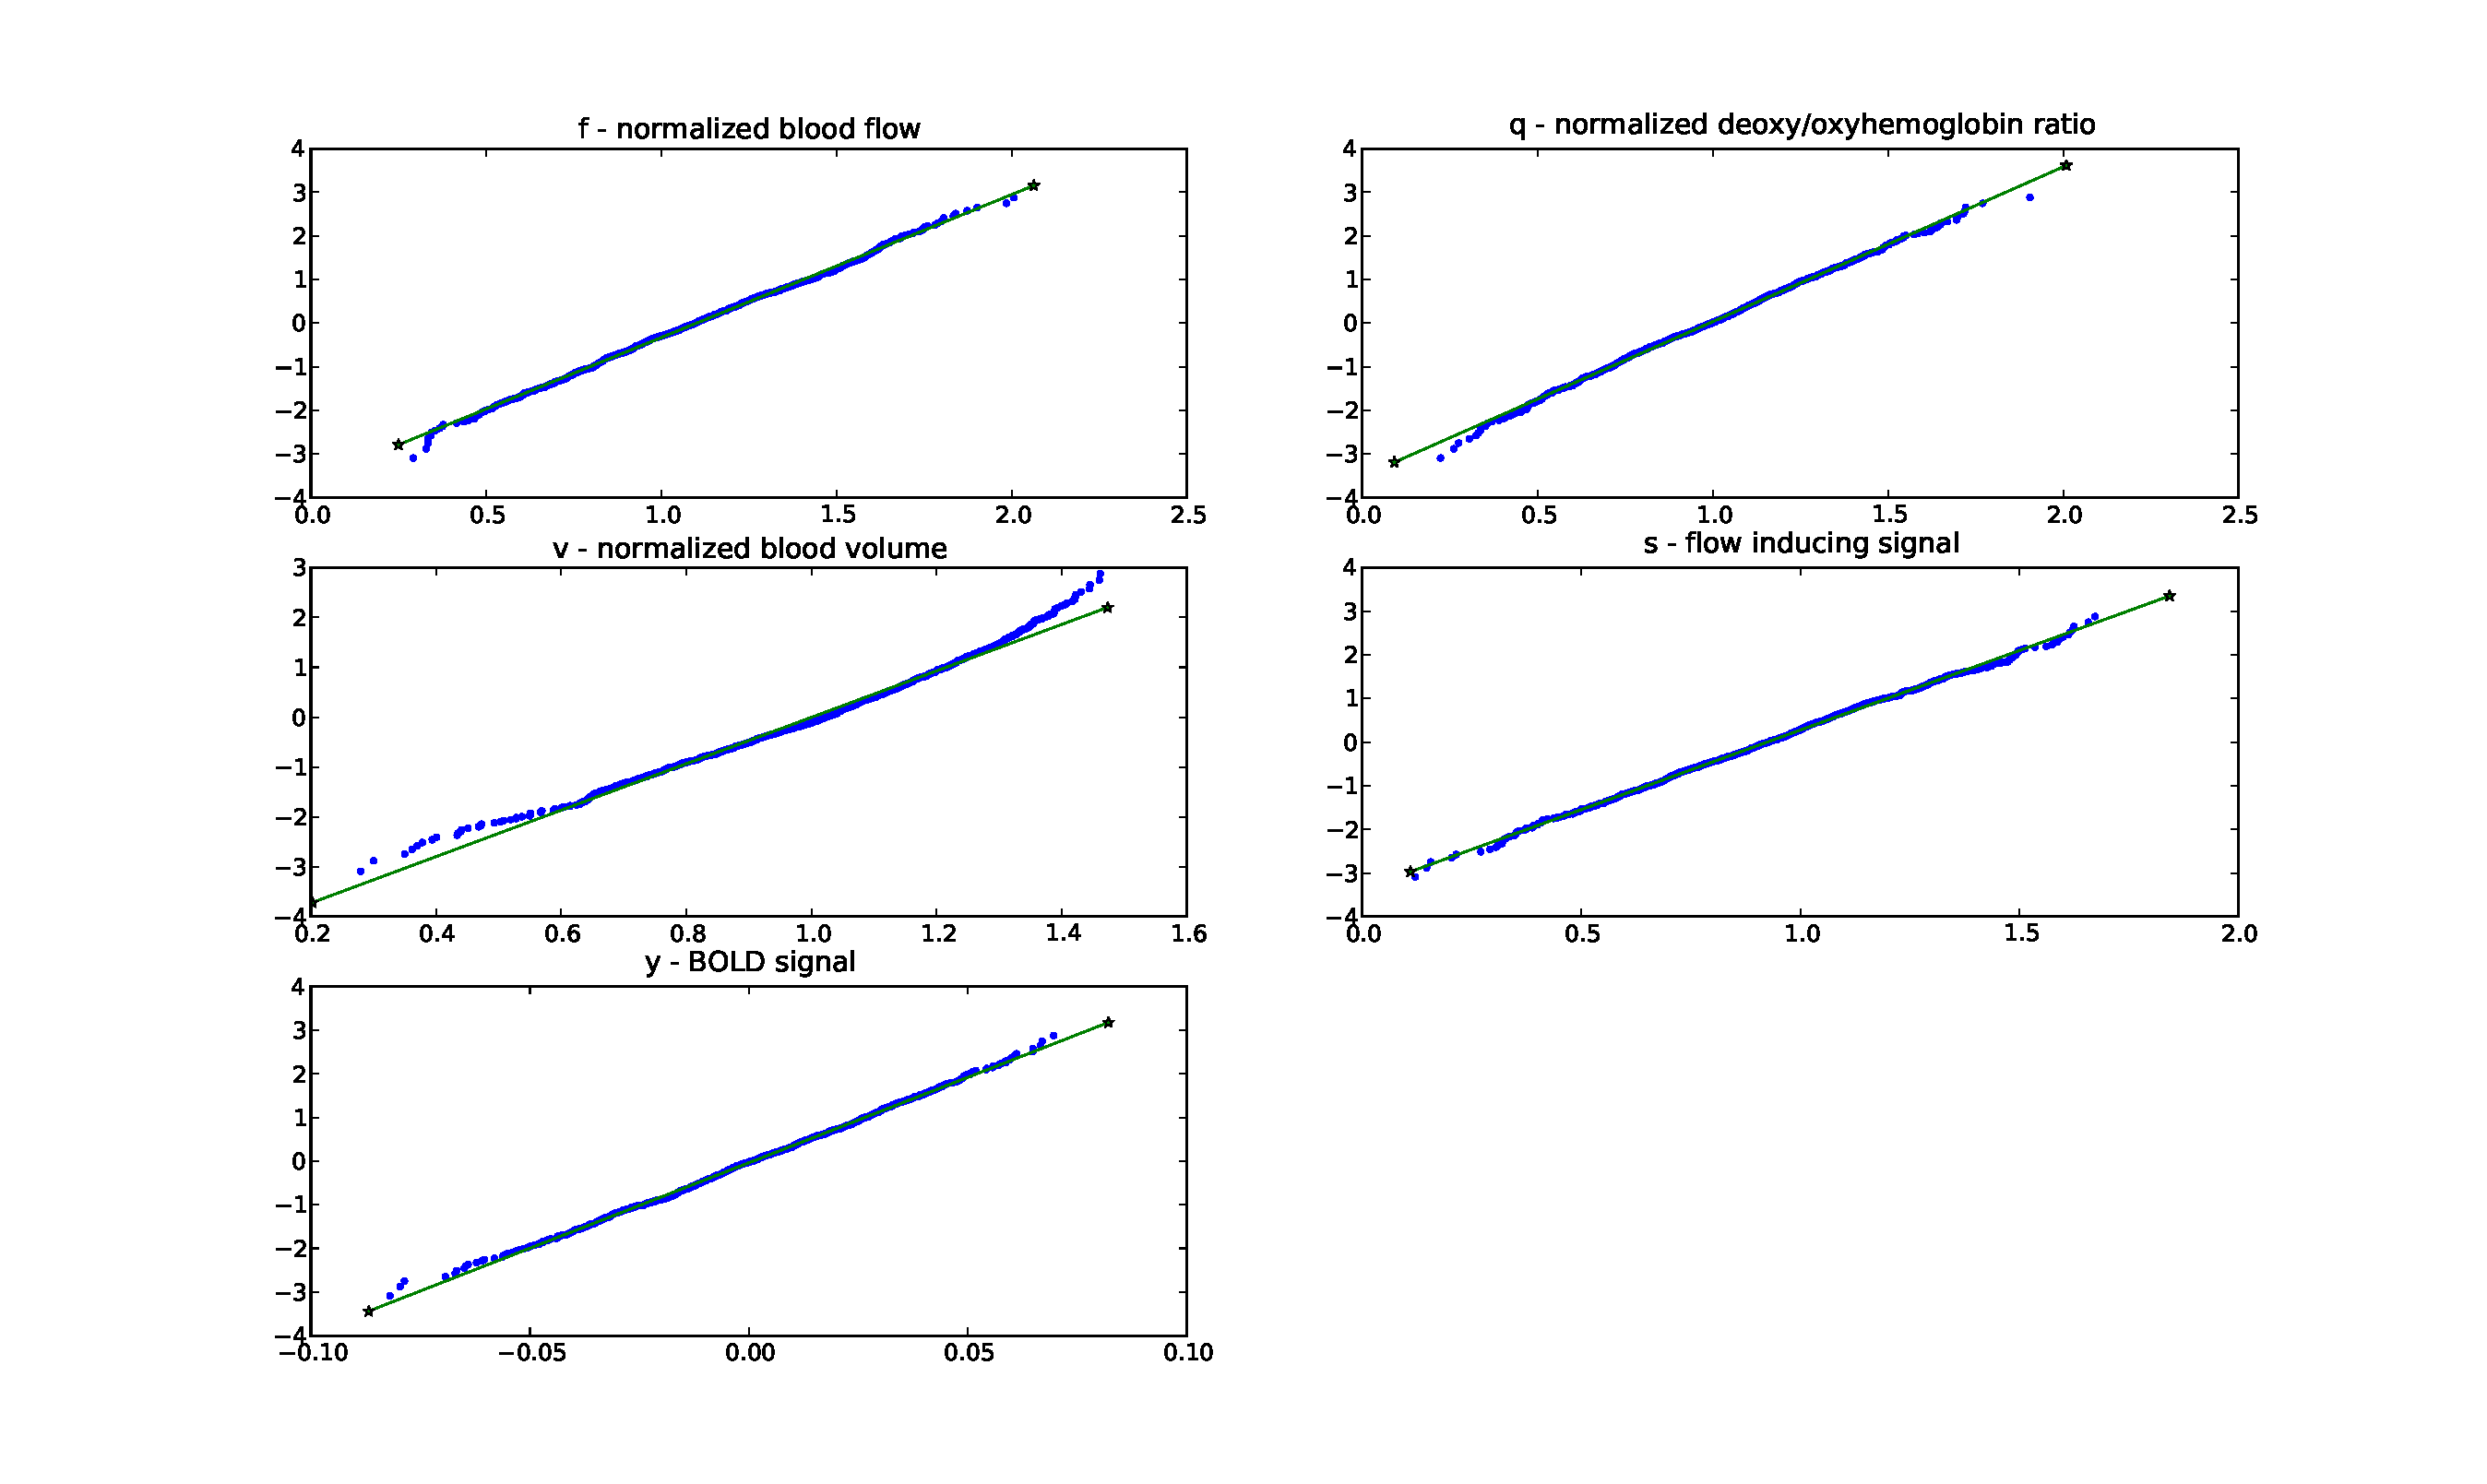
\includegraphics[trim=6cm .75cm 6cm .75cm,width=16cm]{images/gauss_step_point1sec_3sigma.pdf}
\caption{Distributions of state variables after simulating for .1s}
\label{fig:transp1s}
\end{figure}

\begin{figure}
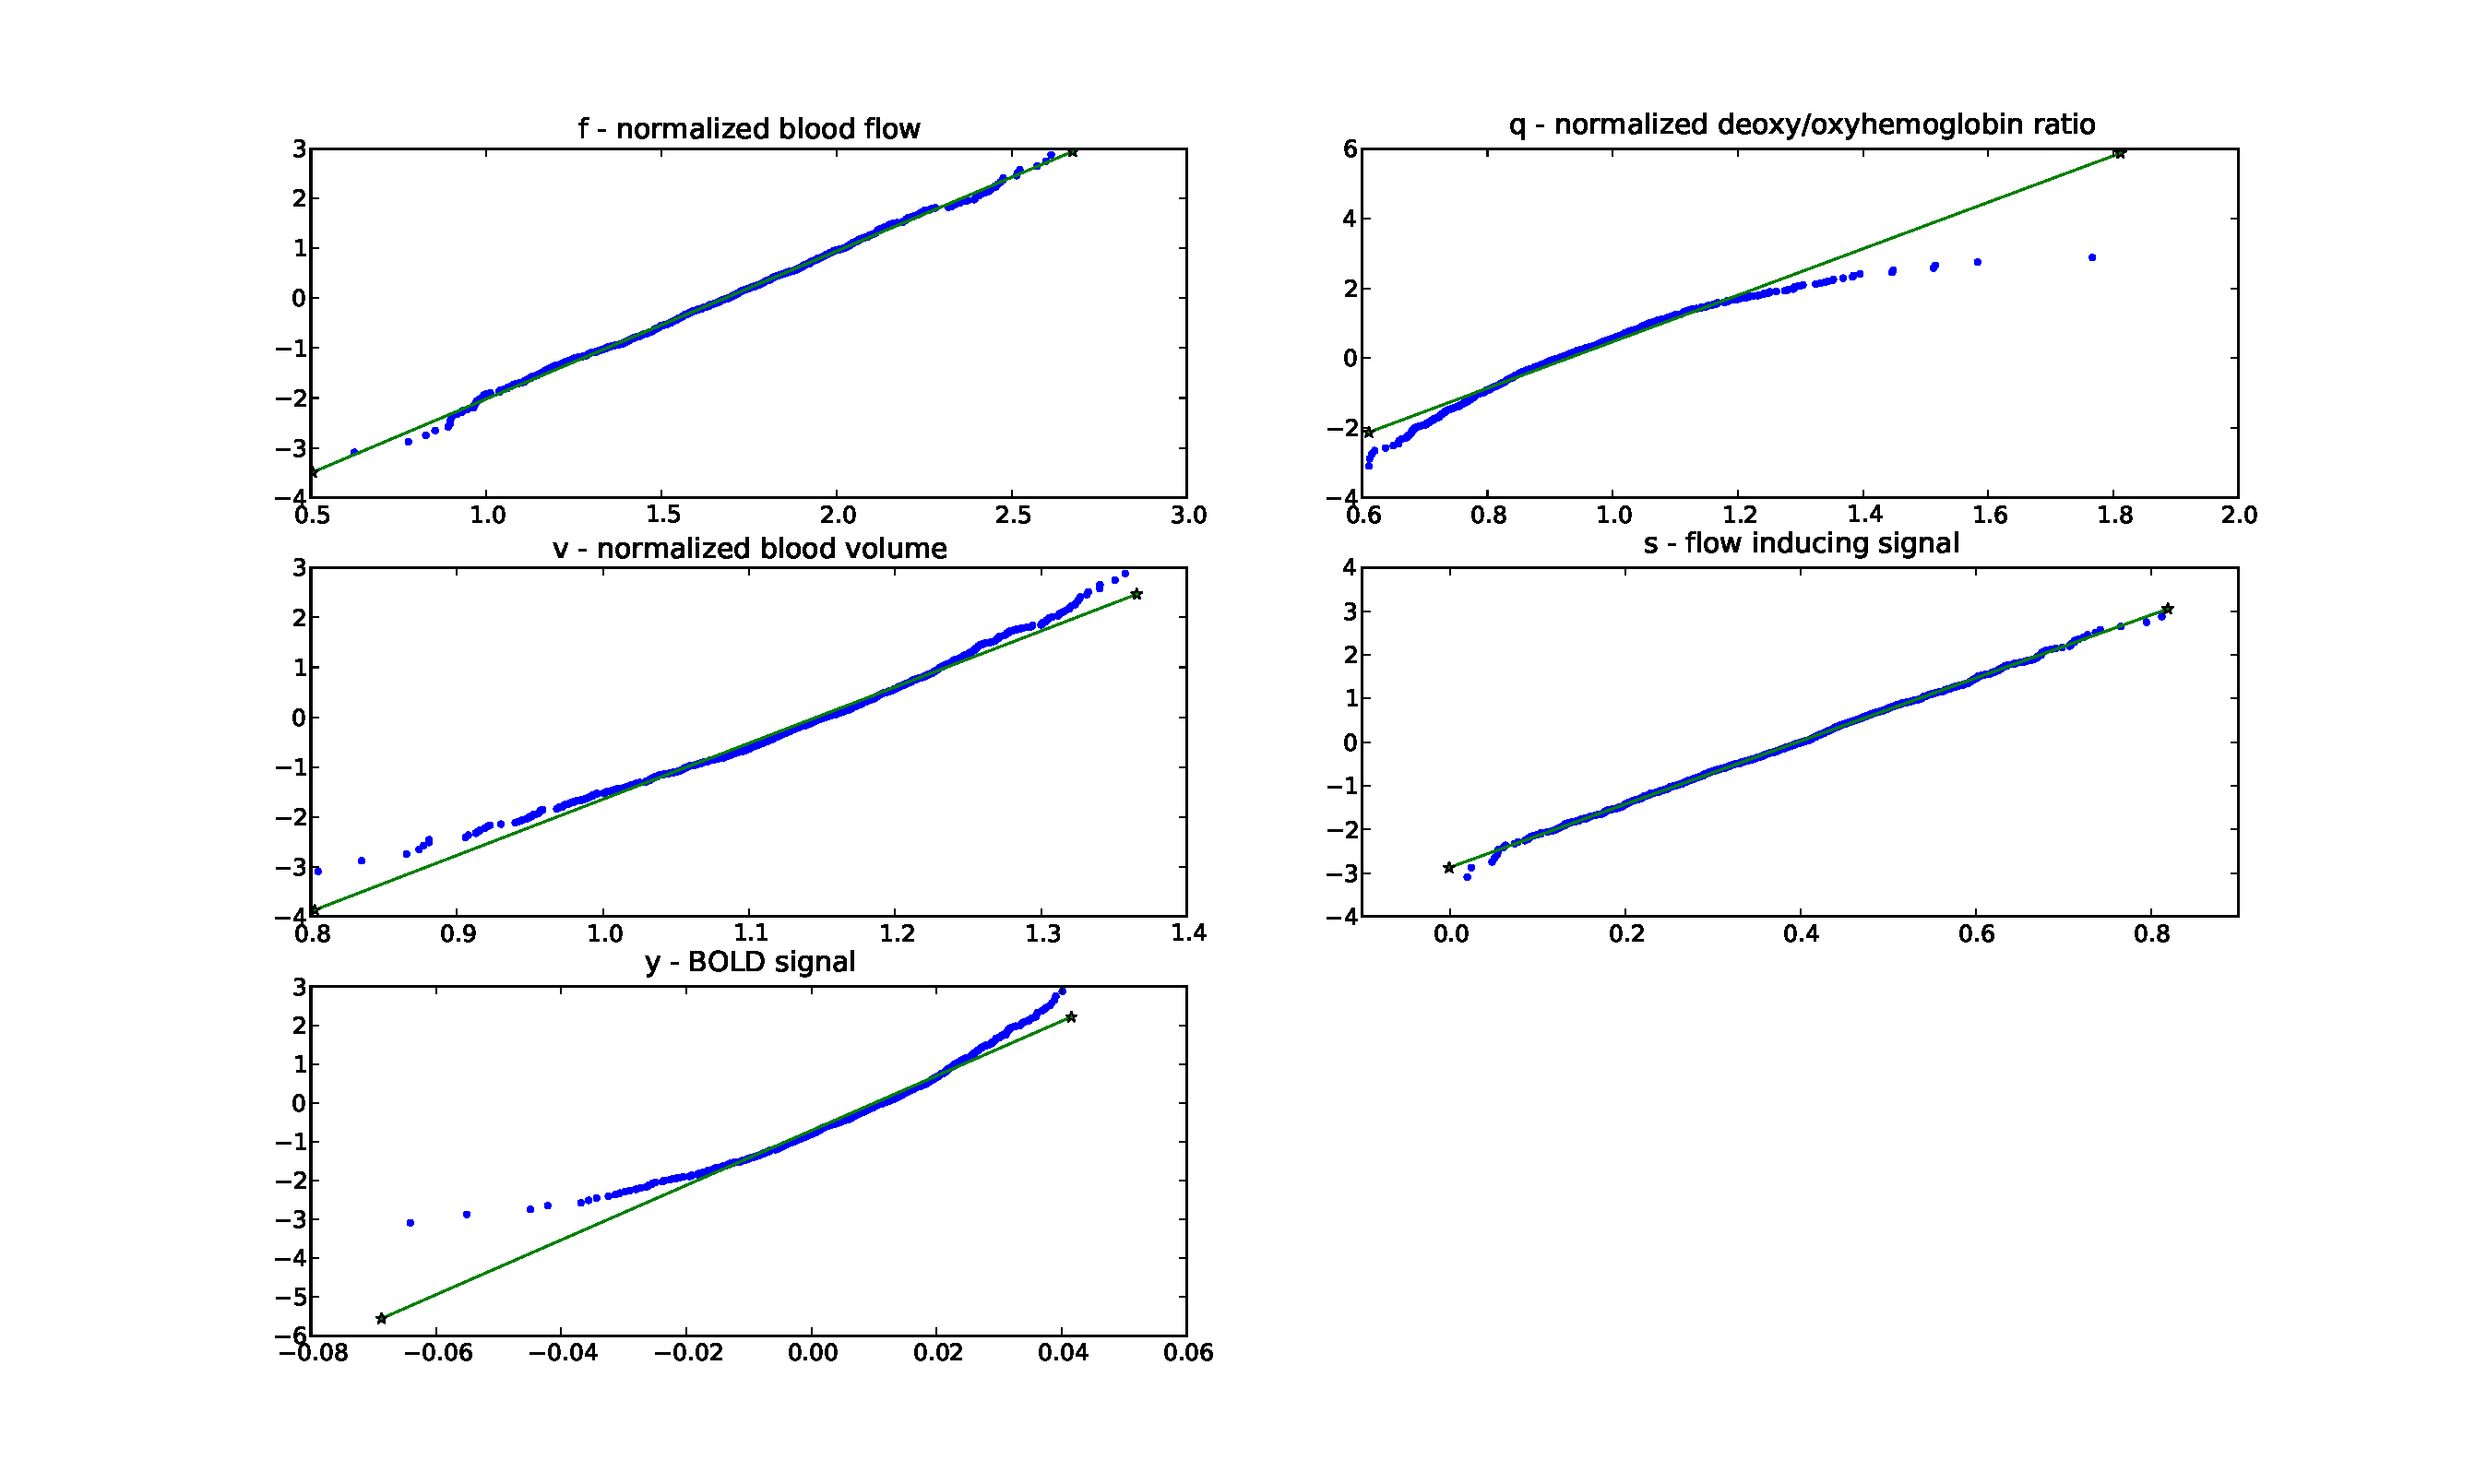
\includegraphics[trim=6cm .75cm 6cm .75cm,width=16cm]{images/gauss_step_1sec_3sigma.pdf}
\caption{Distributions of state variables after simulating for 1s}
\label{fig:trans1s}
\end{figure}

\section{Variational Filtering}
\cite{Friston2008}, \cite{Friston2008b}

\section{Hybrid Methods}
A large number of hybrid methods have been tried, in order to elicit 
parameter estimates from the BOLD model. \cite{Vakorin2007},
\cite{Johnston2007}, \cite{Hu2009}

\section{Conclusion}
In summary, several other approaches could be taken 
